% Homework 13.tex 

\documentclass{article}
\usepackage{graphicx} % for figures
\usepackage{float}
\usepackage[export]{adjustbox}
\usepackage{fancyhdr}
\begin{document}

\title{Homework 11 - Physics 240\\
		System of Spring and Matrix Inversion}
\author{Tin Tran}

\maketitle

\section{Introduction}
The purpose of this excercise is to a fit (linear, power-law, or exponential) to a set of data, calculate the fit parameters, uncertainty, and $\chi ^2$ value. 
\section{Discussion and data}
I got my data from NASA giss, specifically the Global annual mean surface air temperature change vs time. After fitting the data, I got the following outputs

\begin{figure}[H]
\centering{
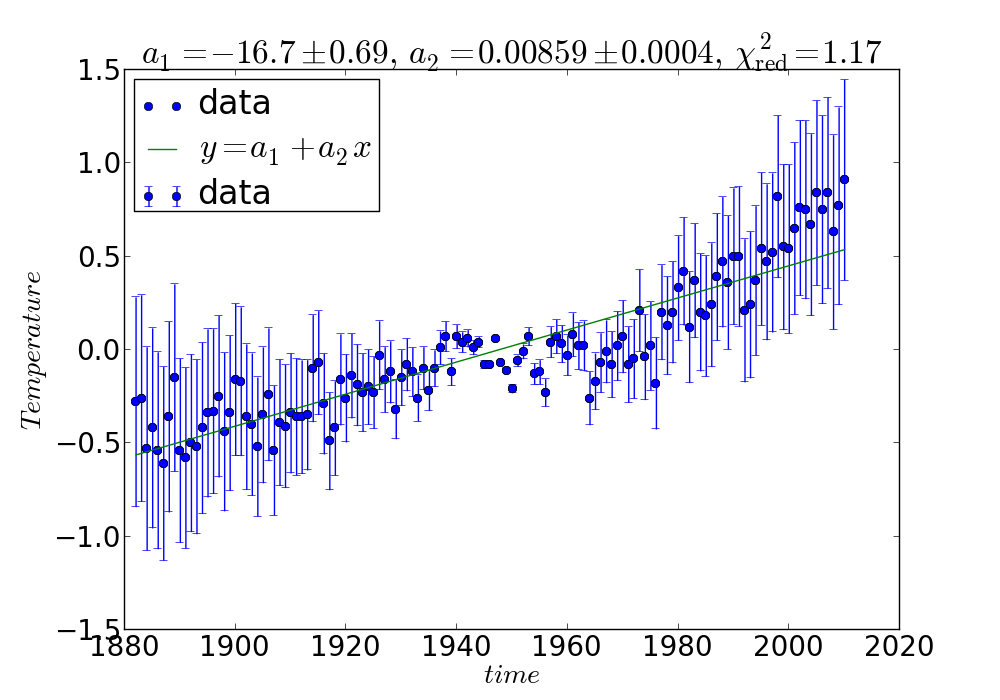
\includegraphics[max size={\textwidth}{\textheight}]{hw13a.png}
\caption{Linear fit of Global Temperature vs time}
}
\end{figure}
As shown, the a$_1$ value is -16.7$\pm$0.69, a$_2$ = 0.00859 $\pm$0.0004, and $\chi ^2$ is 1.17. Because my data doesn't include $\sigma_i$ I picked $\sigma_i$ = $\sigma_o$ = 0.15, which is reasonable for my data. Note that this is a linear fit, for the reason is that my data was less than 1 and some are negative, therefore doing a log(y) or ln(y) for the power-law or exponential was not a good idea because the data would then scatter all over the place like the following figure.
\begin{figure}[H]
\centering{
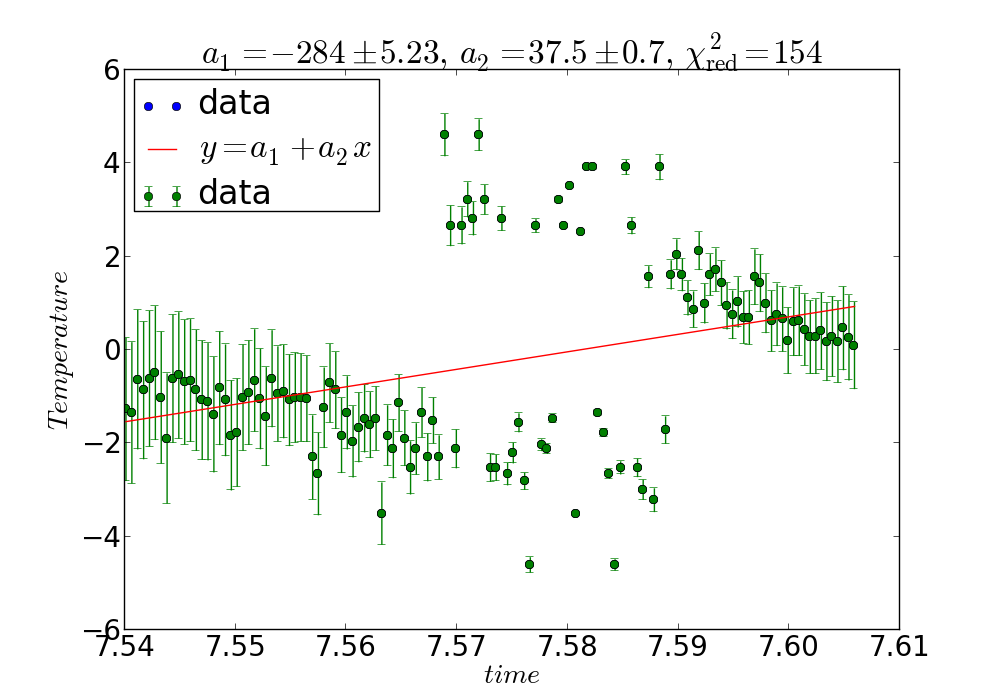
\includegraphics[max size={\textwidth}{\textheight}]{hw13b.png}
\caption{Power-law fit of Global Temperature vs time}
}
\end{figure}
The data scattered all over the place as the result of taking log of something less than 1, which then turns into a negative number.\\\\
If I just take the log without first moving the negative sign out, then some data point can't be computed because of log(negative) and I get the following plot.
\begin{figure}[H]
\centering{
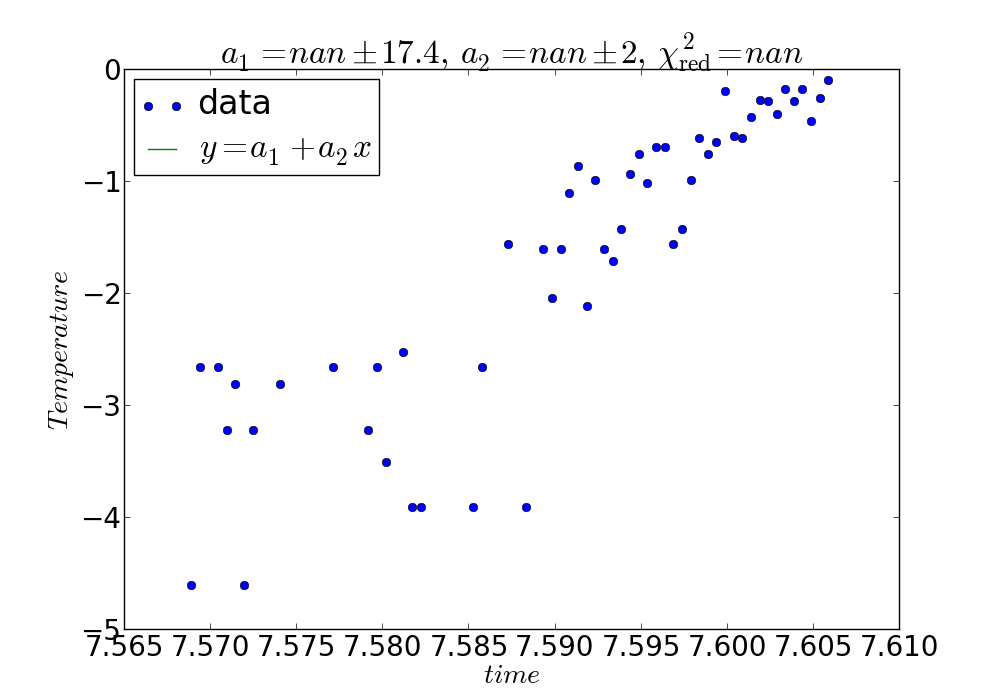
\includegraphics[max size={\textwidth}{\textheight}]{hw13c.png}
\caption{Power-law fit of Global Temperature vs time}
}
\end{figure}
In which none of the parameters were calculated. Therefor for this set of data, the Linear-fit is the best representation of the data. Even on NASA's website the plot is similar to mine.
\end{document}